
Así como existe una infinidad de reacciones químicas en el mundo, existen una infinidad de enzimas en la naturaleza. Intentar estudiarlas sin un orden claro sería todo un caos. Para evitar esto conviene tener una forma estándar de identidicar a las enzimas. 

Durante los inicios del estudio de las enzimas era común nombrarlas en base a sus \emph{características observables}. Por ejemplo, en 1932, Otto Warburg y Walter Christian aislaron una enzima a partir de levadura usada en producción de cerveza, y dado el color amarillento de tal enzima, decidieron nombrarla Enzima Amarilla\footnote{Completos genios}. Unos años después, en 1938, Erwin Haas aisló otra enzima con coloración amarilla a partir de levadura, por lo que la Enzima Amarilla de Otto y Walter pasó a llamarse la Vieja Enzima Amarilla (Old Yellow Enzima, OYE)\citep{williamsNewUsesOld2002}. Hoy día este par de enzimas son catalogadas como flavoproteínas, un amplio grupo de enzimas que utiliza FAD como cofactor, lo que le da a todas estas enzimas un color amarillo/verdoso. Intentar catalogar estas enzimas en base a su color sería claramente poco eficaz, y ejemplifica porqué utilizar características observables no es un buen método de clasificación.

Otra forma que ha sido utilizada para identificar a las enzimas han sido los \emph{nombres comunes}. Este nombre común usualmente se forma colocando primero el \emph{sustrato} sobre el que actua la enzima y luego la \emph{reacción} que lleva a cabo, añadiendo el \emph{sufijo -asa} a la reacción. Tomemos de ejemplo la \emph{NAD\textsuperscript{+} oxidorreductasa}, cuyo nombre se compone primero del sustrato, el \emph{NAD\textsuperscript{+}}, y luego la reacción, \emph{oxidorreducción}, añadiendo \emph{-asa} a al segundo término. Sin embargo, esto jamás fue un sistema estandarizado, por lo que tenemos enzimas como la aldolasa, cuyo nombre es poco descriptivo.

Con el objetivo de reducir tanta confusión, la \acrfull{iubmb}, específicamente su Comisión de Enzimas, estableció un sistema más lógico para denominar y numerar a las enzimas, y este sistema se ha convertido en el más utilizado hasta día de hoy.

Este sistema \emph{clasifica a las enzimas} primero que nada en base al \emph{tipo de reacción} que estas catalizan, lo que genera \emph{7 clases principales}:

\begin{enumerate}
    \item Oxidorreductasas
    \item Transferasas
    \item Hidrolasas
    \item Liasas
    \item Isomerasas
    \item Ligasas
    \item Translocasas\footnote{Esta una clase reciente, añadida apenas en 2018}
\end{enumerate}

Esto sigue sin ser suficiente para la enorme cantidad y variedad de enzimas que existen, por lo que cada una de estas clases se divide a su vez en subclases y subsubclases. Intentar navegar por tantos grupos distintos sería igualmente un caos sin una guía o mapa con el cual guiarse. Afortunadamente, la Comisión de Enzimas estableció también, el Número EC (o EC number), el cuales un identificador único para cada enzima que justamente sirve de guía a través de estas clases y subclases.

Si bien existen otras formas de clasificar a las enzimas, la propuesta por el \acrshort{iubmb} es la más utilizada, por lo que es la que se estudiará principalmente. 

Sin embargo, antes de avanzar es importante dejar un detalle en claro, y es que este sistema de clasificación \emph{no toma en cuenta la cadena de aminoácidos} que compone a la enzima. Tomemos de ejemplo la amilasa, una enzima encargada de hidrolizar glucosa. En el ser humano esta enzima es producida en la saliva y en el pancreas, y aunque en ambos casos llevan a cabo la misma reacción y se les da el mismo número EC, la composición de aminoácidos de cada una es algo diferente, esto porque están en lugares con características diferentes (pH diferente, por ejemplo). De igual manera, la cadena de aminoacidos de la amilasa de una persona no será exactamente igual a la de otra, así como la de un ser humano no será igual a la de otros animales. Este detalle es secundario cuando uno apenas aprende lo básico sobre enzimas, pero es bastante relevante en tareas más avanzadas, como la purificación de enzimas o la producción de enzimas recombinantes.



    \section{Grupos principales de enzimas}\label{sec:clases_de_enzimas}

Como se mencionó antes, la primera división de las enzimas se da en base a la reacción que catalizan. Los nombres de estas clases son bastante autoexplicativos, pero conviene explorarlos un poco.

\subsection{Oxidorreductasas}

Estas enzimas llevan a cabo reacciones de oxido-reducción. Recordemos que estas reacciones consisten en 

    \begin{figure}[H]
    \centering
    {
    \chemnameinit{\chemfig{CH_3-C(-[6]H)(-[2]{\color{red}H})-O{\color{red}H}}}
    \schemestart
        \chemname{\chemfig{CH_3-C(-[6]H)(-[2]{\color{red}H})-O{\color{red}H}}}{\small\bfseries Etanol}
        \arrow(.base east--.base west){-U>[NAD+][NAD{\color{red}H} + {\color{red}H+}][][0.35][60]}[,2.5] 
        \chemname{\chemfig{CH_3-C(-[7]H)=[1]O}}{\small\bfseries Acetaldehido}
    \schemestop
    \chemnameinit{}
    \vspace*{1em} \par
    }
    \rule{\linewidth}{0.2pt}
    \caption[Oxidación del etanol en acetaldehido por la alcohol deshidrogenasa]{Reacción catalizada por la alcohol deshidrogenasa (EC 1.1.1.). Aquí la enzima utiliza el NAD\textsuperscript{+} como cofactor para oxidar el etanol, esto al eliminar de este 2 átomos de hidrógeno y 2 electrones, lo que transforma al etanol en acetaldehido. La alcohol deshidrogenasa está presente en nuestro hígado, y hoy día el principal uso que hacemos de ella es para el metabolismo de bebidas alcohólicas.}
    \label{fig:reaccion_alcohol_deshidrogenasa}
\end{figure}

\marginpar{\resumebox{dato}{\sci{Homo ebrius}}{\footnotesize La evolución de la enzima alcohol deshidrogenasa en humanos y otros homínidos ha sido relacionada con el inicio de consumo de frutas ligeramente fermentadas hace 100 millones de años\citep{carriganHominidsAdaptedMetabolize2015}}}

\subsection{Transferasas}

Las transferasas llevan a cabo transferencias de grupos funcionales entre moléculas.

\begin{figure}[H]
    \centering
    {\schemestart
        \chemfig{}
    \schemestop \vspace*{1em} \par}
    \rule{\linewidth}{0.2pt}
    \caption{Eq}
    \label{fig:reaccion}
\end{figure}

\subsection{Hidrolasas}

Las hidrolasas son enzimas que llevan a cabo esciciones en las moléculas con la ayuda de moléculas de agua, las cuales sirven como receptoras o donadoras de electrones u átomos de oxígeno.

\begin{figure}[H]
    \centering
    {\schemestart
        \chemfig{}
    \schemestop \vspace*{1em} \par}
    \rule{\linewidth}{0.2pt}
    \caption{Eq}
    \label{fig:reaccion}
\end{figure}

\subsection{Liasas}

Las liasas realizan esciciones como las hidrolasas, sin embargo, estas hacen uso de moléculas de agua necesariamente.

    \begin{figure}[H]
    \centering
    {\chemnameinit{\chemfig{{\color{red}H}-C(=[2]O)-CH_3}}
    \schemestart
        \chemname{\chemfig{{\color{blue}^{-}OOC}-C(=[2]O)-CH_3}}{\small\bfseries Piruvato}
        \arrow(.base east--.base west){-U>[{\color{red}H}][][][0.3][60]}[,2]
        \chemfig{{\color{blue}C} | {\color{blue}O_2}}
        \+
        \chemname{\chemfig{{\color{red}H}-C(=[2]O)-CH_3}}{\small\bfseries Acetaldehido}
    \schemestop
    \chemnameinit{}
    \vspace*{1em}
    \par}
    \rule{\linewidth}{0.2pt}
    \caption[Descarboxilación del piruvato en acetaldehido por la piruvato descarboxilasa]{Reacción catalizada por la piruvato descarboxilasa (EC 4.1.1.1). Esta retira el grupo carboxilo (\ce{COOH}), reacción llamada descarboxilación y de donde proviene el nombre descarboxilasa. Tras esto un átomo de hidrógeno toma el lugar del grupo carboxilo.}
    \label{fig:reaccion_piruvato_descarboxilasa}
\end{figure}

\subsection{Isomerasas}

Las isomerasas llevan a cabo el reordenamiento de moléculas, por ejemplo, rotando sus grupos funcionales.

    \begin{figure}[H]
    \centering
    {
    \chemnameinit{\chemfig{^{-}OOC-[7]C(-[5]H)=C(-[7]{\color{red}H})-[1]{\color{blue}C}|{\color{blue}OO^{-}}}}
    \schemestart
        \chemname{\chemfig{^{-}OOC-[7]C(-[5]H)=C(-[7]{\color{red}H})-[1]{\color{blue}C}|{\color{blue}OO^{-}}}}{\small\bfseries Maleato}
        \arrow{<->>}
        \chemname{\chemfig{^{-}OOC-[7]C(-[5]H)=C(-[1]{\color{red}H})-[7]{\color{blue}C}|{\color{blue}OO^{-}}}}{\small\bfseries Fumarato}
    \schemestop
    \chemnameinit{}
    \vspace*{1em} \par}
    \rule{\linewidth}{0.2pt}
    \caption[Isomerización del maleato en fumarato por la maleato isomerasa]{Reacción catalizada por la maleato isomerasa (EC 5.2.1.1). Esta enzima lleva a cabo una reacción de isomeración, o sea, realiza un cambio en el ordenamiento de los átomos del sustrato, el maleato, y que genera un isómero del sustrato, fumarato.}
    \label{fig:reaccion_maleato_isomerasa}
\end{figure}

\subsection{Ligasas}

Las ligasas llevan a cabo la unión de moléculas.

    \begin{figure}[H]
    \centering
    {
    \chemnameinit{\chemfig{{\color{blue}^{-}OOC}-C(=[2]O)-CH_3}}
    \schemestart
        \chemname{\chemfig{^{-}OOC-C(=[2]O)-CH_3}}{\small\bfseries Piruvato}
        \+
        \chemfig{{\color{red}C} | {\color{red}O_2}}
        \arrow(.base east--.base west){-U>[ATP][ADP + Pi][][0.3][60]}[,2]
        \chemname{\chemfig{^{-}OOC-C(=[2]O)-CH_2-{\color{red}COO^{-}}}}{\small\bfseries Oxalacetato}
    \schemestop
    \chemnameinit{}
    %\vspace*{1em}
    \par
    }
    \rule{\linewidth}{0.2pt}
    \caption[Carboxilación del piruvato en oxalacetato por la piruvato carboxilasa]{Reacción catalizada por la piruvato carboxilasa (EC 6.4.1.1). En este ejemplo la enzima añade una molécula de dióxido de carbono (\ce{CO2}) a una molécula de piruvato, lo que genera oxalacetato. Este proceso de añadir un grupo carboxilo se conoce como carboxilación, y es el proceso opuesto a la descarboxilación viso en la \autoref{fig:reaccion_piruvato_descarboxilasa}. }
    \label{fig:reaccion_piruvato_carboxilasa}
\end{figure}

\subsection{Translocasas}

Este grupo, recien añadido en 2018, engloba aquellas enzimas encargadas de transportar moléculas de un medio dado a otro. Por ejemplo, las enzimas de la membrana celular que se dedican a transportar iones de un lado a otro de la membrana.

\begin{figure}[H]
    \centering
    {\schemestart
        \chemfig{}
    \schemestop \vspace*{1em} \par}
    \rule{\linewidth}{0.2pt}
    \caption{Eq}
    \label{fig:reaccion}
\end{figure}



\section{Número EC (EC Number)}

El \emph{número EC}, o EC number en ingles, es un código de 4 dígitos que se el asigna a cada enzima, donde cada dígito corresponde a un ``escalón''.

\begin{figure}[H]
    \centering
    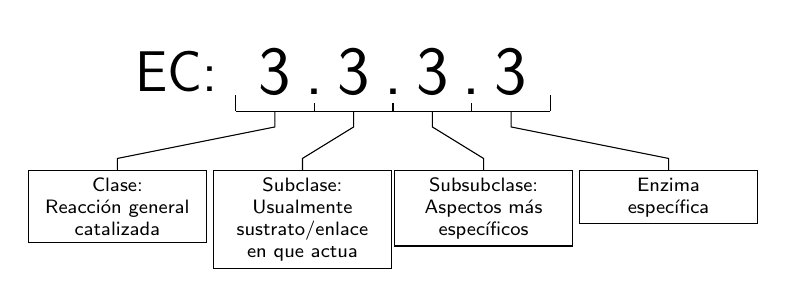
\begin{tikzpicture}
    
    \node[draw=none, node font=\huge\sffamily] at (-1.25,0) {EC:};
    \node[draw=none, node font=\Huge\sffamily] at (0,0) {3};
    \node[draw=none, node font=\Huge\sffamily] at (0.5,-0.25) {.};
    \node[draw=none, node font=\Huge\sffamily] at (1,0) {3};
    \node[draw=none, node font=\Huge\sffamily] at (1.5,-0.25) {.};
    \node[draw=none, node font=\Huge\sffamily] at (2,0) {3};
    \node[draw=none, node font=\Huge\sffamily] at (2.5,-0.25) {.};
    \node[draw=none, node font=\Huge\sffamily] at (3,0) {3};
  
    \draw (-0.5,-0.5) -- (3.5,-0.5);
    \draw (-0.5,-0.5) -- (-0.5, -0.3);
    \draw (0.5,-0.5) -- (0.5, -0.4);
    \draw (1.5,-0.5) -- (1.5, -0.4);
    \draw (2.5,-0.5) -- (2.5, -0.4);
    \draw (3.5,-0.5) -- (3.5, -0.3);

    \node[anchor=north, draw, text width=8em, align=center, node font=\scriptsize\sffamily] (clase) at (-2,-1.25) {Clase:\\Reacción general catalizada};
    \node[anchor=north, draw, text width=8em, align=center, node font=\scriptsize\sffamily] (subclase) at (0.35,-1.25) {Subclase:\\Usualmente sustrato/enlace en que actua};
    \node[anchor=north, draw, text width=8em, align=center, node font=\scriptsize\sffamily] (subsubclase) at (2.65,-1.25) {Subsubclase:\\Aspectos más específicos};
    \node[anchor=north, draw, text width=8em, align=center, node font=\scriptsize\sffamily] (enzima) at (5,-1.25) {Enzima\\específica};

    \draw (0,-0.5) --(0,-0.7) -- (-2,-1.1) -- (clase.north);
    \draw (1,-0.5) --(1,-0.7) -- (0.35,-1.1) -- (subclase.north);
    \draw (2,-0.5) --(2,-0.7) -- (2.65,-1.1) -- (subsubclase.north);
    \draw (3,-0.5) --(3,-0.7) -- (5,-1.1) -- (enzima.north);

\end{tikzpicture}
    \label{fig:ec_number}
\end{figure}

Por ejemplo, el \emph{primer dígito} corresponde a la \emph{clase principal}, las 7 que se estudiaron anteriormente (\autoref{sec:clases_de_enzimas}). El \emph{segundo dígito} corresponde a una de las \emph{subclases} existentes dentro de la clase principal las cuales describen el sustrato o enlace sobre el que actua la enzima. Lo mismo sucede con el tercer dígito que es una subclase dentro de la subclase anterior. El cuarto dígito, ahora si, es un identificador propio de cada enzima.

Este sistema se puede entender como un arbol, donde las ramas se van dividiendo en otras ramas. Aquí el número EC sirve pues como una guia sobre qué grupos seguir. Una forma visualizar esto es a través de la \textbf{\href{https://www.brenda-enzymes.org/ecexplorer2.php?browser=1}{base de datos BRENDA}}, que cuenta con un explorador de las diferentes clases de enzima.

\section{Identificador UniProt}

Como se mencionó anteriormente, la clasificación más común de enzimas se basa en la reacción que catalizan, sin embargo, esto no significa que enzimas que compartan número EC compartan también la misma cadena de aminoácidos. El \emph{identificador UniProt} es otro código el cual si que se asigna en \emph{base a la cadena de aminoácidos}.

